% \levelC{Objective}
In chapter \ref{sec:evalmodels}, it was observed that achieving 0.6 accuracy on file fragment classification using 28 classes was a difficult task to the considered models. In other studies results \cite{hiester_file_2018} \cite{sportiello_context-based_2012} \cite{amirani_feature-based_2013} \cite{maslim_distributed_2014} and on initial tests, the achieved accuracy for small number of classes was considerably higher. Hiester \cite{hiester_file_2018}, for instance, achieves an accuracy of 98\% using four classes.

This chapter investigates how does the accuracy of the considered models change in relation to the number of classes in the dataset.


% \levelC{Dataset}
This study uses the Govdocs1 dataset \cite{garfinkel_bringing_2009}, which was fully downloaded and its files were grouped by extension. This dataset has files with 63 different extensions. The 33 extensions with less than 200 files were discarded. The  ``text'' and ``unk'' extensions were discarded because files with these extensions use multiple formats and they do not correspond to a single file type. From the remaining 28 extensions, listed in table \ref{tab:govdocs1}, 200 files of each were randomly selected, 100 to use in the training dataset and 100 to use in the validation dataset.

% \begin{table}[!ht]
    \centering
    \caption{Govdocs1 dataset}
    \label{tab:govdocs1}
\begin{tabular}{|l|l|l|}
\hline
Extension & Number of files & Number of blocks \\ \hline
                                                  \hline
pdf       & 231232          & 268071071    \\ \hline
html      & 214568          & 25710908     \\ \hline
jpg       & 109233          & 73242253     \\ \hline
txt       & 78286           & 99435540     \\ \hline
doc       & 76616           & 60654930     \\ \hline
xls       & 62635           & 58718224     \\ \hline
ppt       & 49702           & 251210471    \\ \hline
gif       & 36302           & 5962516      \\ \hline
xml       & 33458           & 16954875     \\ \hline
ps        & 22015           & 56547464     \\ \hline
csv       & 18360           & 6843009      \\ \hline
gz        & 13725           & 17748905     \\ \hline
log       & 9976            & 8467819      \\ \hline
eps       & 5191            & 5756138      \\ \hline
% unk       & 5186            & 2983922      \\ \hline
png       & 4125            & 2207489      \\ \hline
swf       & 3476            & 3798321      \\ \hline
dbase3    & 2601            & 38972        \\ \hline
pps       & 1619            & 7432480      \\ \hline
rtf       & 1125            & 958239       \\ \hline
kml       & 993             & 309422       \\ \hline
kmz       & 943             & 549462       \\ \hline
% text      & 839             & 1527118      \\ \hline
hlp       & 659             & 8692         \\ \hline
f         & 602             & 94543        \\ \hline
sql       & 462             & 244634       \\ \hline
wp        & 364             & 87643        \\ \hline
dwf       & 299             & 85500        \\ \hline
java      & 292             & 14530        \\ \hline
pptx      & 215             & 1151796      \\ \hline
% fits      & 182             & 678128       \\ \hline
% tmp       & 180             & 28426        \\ \hline
% tex       & 163             & 10520        \\ \hline
% docx      & 163             & 65969        \\ \hline
% troff     & 110             & 8020         \\ \hline
% bmp       & 72              & 62686        \\ \hline
% sgml      & 62              & 44138        \\ \hline
% gls       & 60              & 517          \\ \hline
% pub       & 55              & 1421         \\ \hline
% xlsx      & 37              & 12910        \\ \hline
% fm        & 25              & 6717         \\ \hline
% zip       & 10              & 31525        \\ \hline
% ttf       & 10              & 1540         \\ \hline
% xbm       & 8               & 578          \\ \hline
% wk1       & 7               & 6493         \\ \hline
% sys       & 7               & 15           \\ \hline
% ileaf     & 4               & 1656         \\ \hline
% exported  & 3               & 324          \\ \hline
% data      & 3               & 1733         \\ \hline
% odp       & 2               & 2384         \\ \hline
% mac       & 2               & 0            \\ \hline
% lnk       & 2               & 2            \\ \hline
% js        & 2               & 36           \\ \hline
% g3        & 2               & 498          \\ \hline
% chp       & 2               & 73           \\ \hline
% 123       & 2               & 434          \\ \hline
% wk3       & 1               & 229          \\ \hline
% vrml      & 1               & 660          \\ \hline
% squeak    & 1               & 25354        \\ \hline
% py        & 1               & 480          \\ \hline
% pst       & 1               & 20           \\ \hline
% icns      & 1               & 0            \\ \hline
% bin       & 1               & 7            \\ \hline
\end{tabular}
\end{table}


========================

% \levelC{Hardware}
The experiments did not take advantage of GPU acceleration and were  conducted on a single computer with 256GB of RAM and with 2 Intel\textregistered Xeon\textregistered E5-2630 v2 processors, with 6 cores each, with 2 hyper-threads per core, or 24 hyper-threads in total. 


% \levelC{Software}
The main software and frameworks used to build the experiments were Python 3.6, Jupyter notebook, Tensorflow 1.14.0, Keras 2.2.4-tf, and Fedora Linux 27.

% repository
The source code for the experiments is available at \sloppy\url{http://github.com/atilaromero/randomness-experiments}.

\levelC{Models}
The same sampling, input, and output details described in section \ref{sec:evalmodels} were used here. The model identified as ``CM'' was selected to be used.

\levelC{Results}
% decrease in accuracy
Figure \ref{fig:nclasses} shows the graph of accuracy versus number of classes for the ``CM'' model. The bottom line indicates, for comparison, what the accuracy would be for a random guessing classifier. An increase in the number of classes appears to be  correlated with a decrease in accuracy. Another relevant aspect of the graph is that the range of the results seems to be smaller when more classes are used.  

This pattern is understandable: as the number of classes grows, the harder the classification problem is, leading to a decrease in accuracy, while the individual contributions of each class to the overall result diminishes, leading to an increase in precision.

This behavior is an important aspect to consider during the evaluation of file fragments studies. As Beebe et al. \cite{beebe_sceadan:_2013} have mentioned, studies that select fewer classes tend to yield higher results. 

Still, with 46\% \todo{check} of samples being misclassified when the number of classes is 28, the question of what are the error sources and how they can be addressed requires attention.

\noindent
\begin{figure*}[htb!]
\centering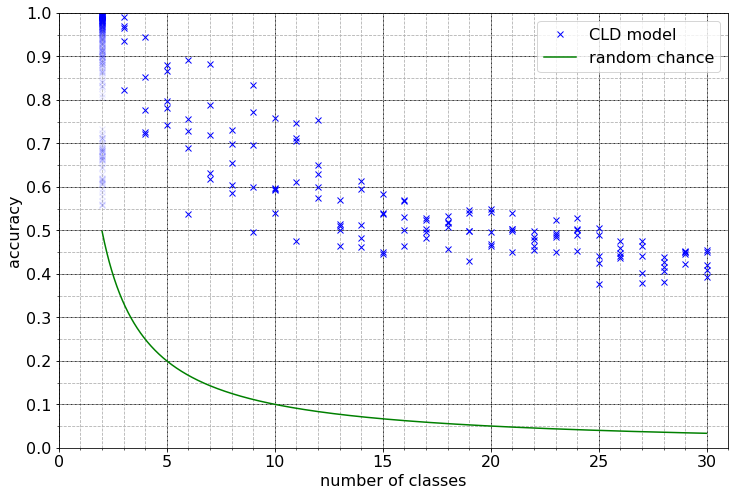
\includegraphics[width=1.0\textwidth]{content/nclasses.png}
\caption{\label{fig:nclasses}Validation accuracy by number of classes}%
\end{figure*}

Figure \ref{fig:dual} shows the graph of the accuracy of each class when compared individually with each one of the others. Generally, file types with higher entropy tend to have lower minima, with the GIF \todo{check} file type being a notable exception. Most of these files use some form of compression, like image files for example. 


\noindent
\begin{figure*}[htb!]
\centering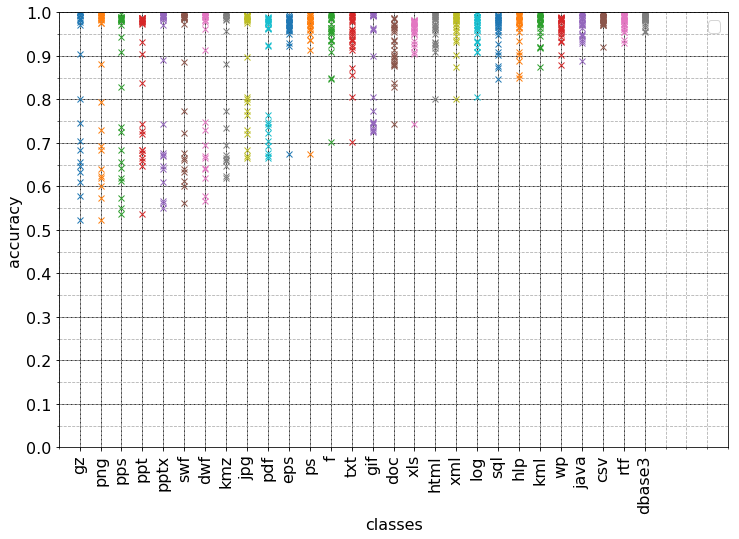
\includegraphics[width=1.0\textwidth]{content/dual.png}
\caption{\label{fig:dual}Validation accuracy of models trained with pair of classes}%
\end{figure*}


The accuracy obtained after the training of models with pairs of classes was used to build a 28x28 matrix, using 0.5 in the main diagonal entries. This number was chosen because a pair of indistinguishable classes would have this accuracy on average. Then, a Principal Component Analysis (PCA) \cite{amirani_new_2008} was used to treat this matrix. The result is shown in figures \ref{fig:pca} and \ref{fig:pca2}. Again some file types with high entropy emerge as a promising group, \todo{check} ``dwf'',
``jpg'',
``pps'',
``ppt'',
``gz'',
``png'',
``pptx'',
``swf'',
``kmz'',
and ``pdf''.

\noindent
\begin{figure*}[htb!]
\centering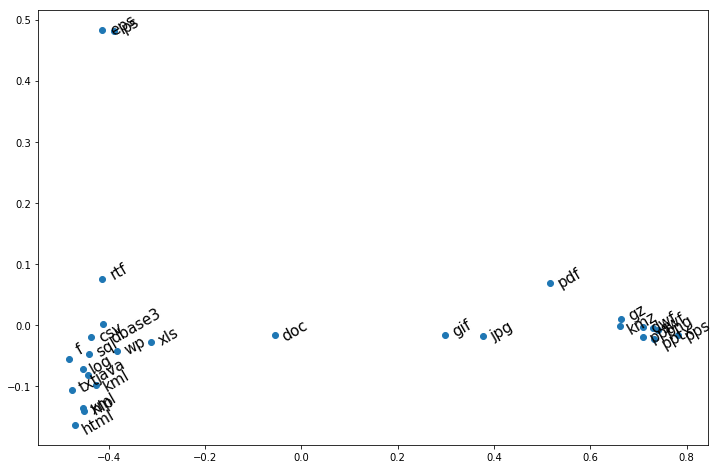
\includegraphics[width=1.0\textwidth]{content/pca.png}
\caption{\label{fig:pca}PCA of accuracy of models trained with pair of classes}%
\end{figure*}


\noindent
\begin{figure*}[htb!]
\centering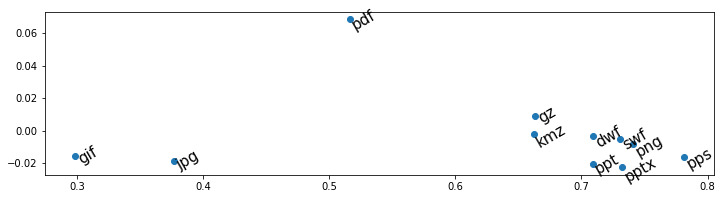
\includegraphics[width=1.0\textwidth]{content/pca2.png}
\caption{\label{fig:pca2}PCA of accuracy of models trained with pair of classes - detail}%
\end{figure*}


% the problem of unseen file types
% \levelC{Limitations and threats to validity}




% \levelC{???}
Several independent models were trained with 2 to 28 extensions from the Govdocs1 dataset. For each number in the range 2 to 28, a random subset of extensions was selected to compose the dataset. Each extension has 200 file samples, half placed in the training dataset and half in the validation dataset. Each dataset was used to train a new model, that should distinguish between the selected subset of extensions in that filtered dataset. This process was repeated five times.



In addition to this sampling of extensions using different quantities of classes, all 378 combinations of pairs of extensions were compared. Each pair was used to compose a dataset and to train a new model for each one, using the same process described in the previous paragraph.


